\documentclass{article}
\usepackage{graphicx}
\usepackage{subcaption}
\usepackage{float}
\graphicspath{ {images/} }
\usepackage{hyperref}
\setcounter{tocdepth}{4}
\setlength\parindent{0pt}
\usepackage[margin=1in]{geometry}
\usepackage{multirow}


\newcommand*{\titleGP}{\begingroup % Create the command for including the title page in the document
\centering % Center all text
\vspace*{\baselineskip} % White space at the top of the page

\rule{\textwidth}{0pt}\vspace*{-\baselineskip}\vspace*{2pt} % Thick horizontal line
\rule{\textwidth}{0pt}\\[\baselineskip] % Thin horizontal line

{\LARGE ~}\\[0\baselineskip] % Title

\begin{figure}[h]
  \centering
  
\includegraphics[scale=0.6]{logo}
\end{figure}


\scshape  % Small caps
\textbf{\LARGE Real-Time Multi-Camera}\\

\vspace*{1\baselineskip}
\textbf{\LARGE 3D Reconstruction}\par

\vspace*{5\baselineskip}

Created by Group 30\\[\baselineskip]
%\vspace*{2\baselineskip}
{\Large Jacek Burys (jsb314) \\ Adam Hosier (ah3114) \\ Rui Liu (rl2414) \\  Ayman Moussa (am5514) \\Kabeer Vohra (kv113) \\  \par} % Editor list

\vfill 

{\scshape 09-January-2017} \\[0.3\baselineskip] % Year published
{\itshape Imperial College London\par} % Editor affiliation

\endgroup}

\begin{document} 

\titleGP
\thispagestyle{empty}

\newpage
\setcounter{page}{1}
\tableofcontents

\newpage
% OLD EXECUTIVE SUMMARY
% COMMENTED OUT, START
\iffalse
\section{Executive Summary}
The ability to capture and record 3D images, and to display them back in real time has multiple use cases today. Through \texttt{Pointify} we have developed a system that utilises Microsoft's proprietary \texttt{Xbox Kinect V2} hardware to stream 3D images based on the depth and colour data from the sensors on the devices in real time, allowing us to reconstruct a 3D model of a scene, that updates live. The user can move around in the scene and view the captured objects from any angle, as well as export this data to edit in third party software. It is a cross-platform service which allows the each component to run on Windows, OS X or Linux operating systems. We achieve this by using services and programming languages that run on all operating systems. Having multiple calibrated \texttt{Kinect V2} cameras allows for a full 360 degree view of the object or scene that is being reconstructed. 
\\\\
The system follows a client-server model, and works as follows:
\\
\subsection{Client}
The client software is responsible for connecting to the \texttt{Kinect V2} sensors, capturing 3D images from these sensors and streaming it to the server, using the following technologies:
\begin{itemize}
\item Industry standard open source computer vision library \texttt{OpenCV} \cite{opencv} to perform matrix operations as efficiently as possible
\item Open source \texttt{libfreenect2} \cite{libfreenect} drivers from OpenKinect to extract the colour and depth camera data from the camera
\item \texttt{AruCo} \cite{aruco} calibration as a module for \texttt{OpenCV} which we use to detect a marker within the scene and use it to calibrate the coordinate spaces of all cameras
\item A custom point cloud structure to hold the 3D images, consisting of a number of colour points in three dimensional space
\item Open-source \texttt{C++11} implementation of \texttt{Socket.IO} \cite{socketio} client to communicate with the server and send the point cloud data when requested
\end{itemize}
\vspace{1mm}
\subsection{Server}
The server is responsible for accepting connections from multiple clients, coordinating and combining their requests and sending the final point cloud to the user:
\begin{itemize}
\item Uses \texttt{Node.js} \cite{node} framework
\item Run using the \texttt{Gulp} \cite{gulp} to automatically deploy the server on \texttt{localhost}
\item Uses \texttt{Socket.IO} \cite{socketio} to communicate with the clients and the viewer as well as to synchronise the frames when taking a picture or streaming
\end{itemize}
\newpage
\subsection{Viewer}
We have also created a front end which serves as the command centre from which all the Kinect clients can be controlled:
\begin{itemize}
\item Uses \texttt{AngularJS} \cite{angular} framework
\item Utilises \texttt{three.js} \cite{three} renderer to display the received point clouds in near real-time
\item Can export current picture or video stream as a \texttt{PLY} file, to use in third party software
\end{itemize}
\subsection{Use cases}
For static imaging there are two main use cases. In manufacturing, it is often the case that people wish to create duplicates of objects they already own. For example drill bits or trimmer attachments. Our system can achieve this by taking a picture and then exporting the \texttt{PLY} file which can be immediately imported into \texttt{AutoCAD} to 3D print the object. For medical reasons, the system can create 360 degree images of the human body and then send it off to remote doctors for an online diagnosis.
\\\\
For live imaging there are two other use cases. During virtual reality gaming it can be useful to be able to map out the scene and work out the distance of the user from certain objects within their room. This could then be used to create live warnings in the virtual reality headset to alert the user when they are about to come into contact with a physical object in their gaming space. Also much like Google street view our system can be used to create a live 3D view of certain points of interest or general roads which can be live streamed over the internet.
\newpage
\fi
% COMMENTED OUT, END

\section{Executive Summary}
% what is is
3D reconstruction is the process of capturing the shape of real-life objects which give us 3D models that we can manipulate and analyse. It is not an easy task and has been an active area of research in Computer Vision. \texttt{Pointify} is a system which allows the user to create a 3D model of a scene by combining data from multiple \texttt{Kinect V2} cameras.
\\
\\
% Kinect
\texttt{Kinect V2} is an example of a 3D scanner. It combines a normal colour camera with a depth camera. The depth and colour information can be used to obtain a \texttt{point cloud}, which is a set of points in some coordinate system. As \texttt{Pointify} makes use of multiple \texttt{Kinect V2} cameras, we have to merge multiple point clouds to reconstruct the 3D scene. Most of the complexity in this process is in finding the transformations that will bring all these point clouds to the same coordinate system, thus making them overlap correctly to form one scene. This is done with the help of a fiducial marker, a special picture which has to be in the field of view of all cameras at the calibration step. With help of \texttt{ArUco} \cite{aruco}, a library for Augmented Reality applications, we can find the necessary transformations.
\\
\\
% how it's working
Our aim was to create an easy to use and user friendly system which can be set up in minutes. It is a distributed system consisting of a server, multiple clients with \texttt{Kinect V2} cameras and a front end which serves as a control centre. The cameras only have to be pointed at the scene and connected to the server, then they can be controlled from the front end, which gives the user an ability to view the resulting models, stream 3D videos and export them as \texttt{PLY} files.
\\
\\
% why we want it, user cases
There are various benefits of having a system such as \texttt{Pointify}. The models created with it can be used for many purposes. For example, one of the main use cases is in manufacturing, when the user wants to recreate an existing object. \texttt{Pointify} has the ability of exporting the model to a \texttt{PLY} format which then can be used in other software to 3D print the object. Also, in recent years we have seen an increasing interest in Virtual and Augmented Reality applications. We are sure \texttt{Pointify} could be useful for creating immersive and realistic virtual worlds based on real objects.
\\
\\

\section{Introduction}
\begin{figure}[h]
\centering
\begin{subfigure}[b]{0.49\textwidth}
  \centering
  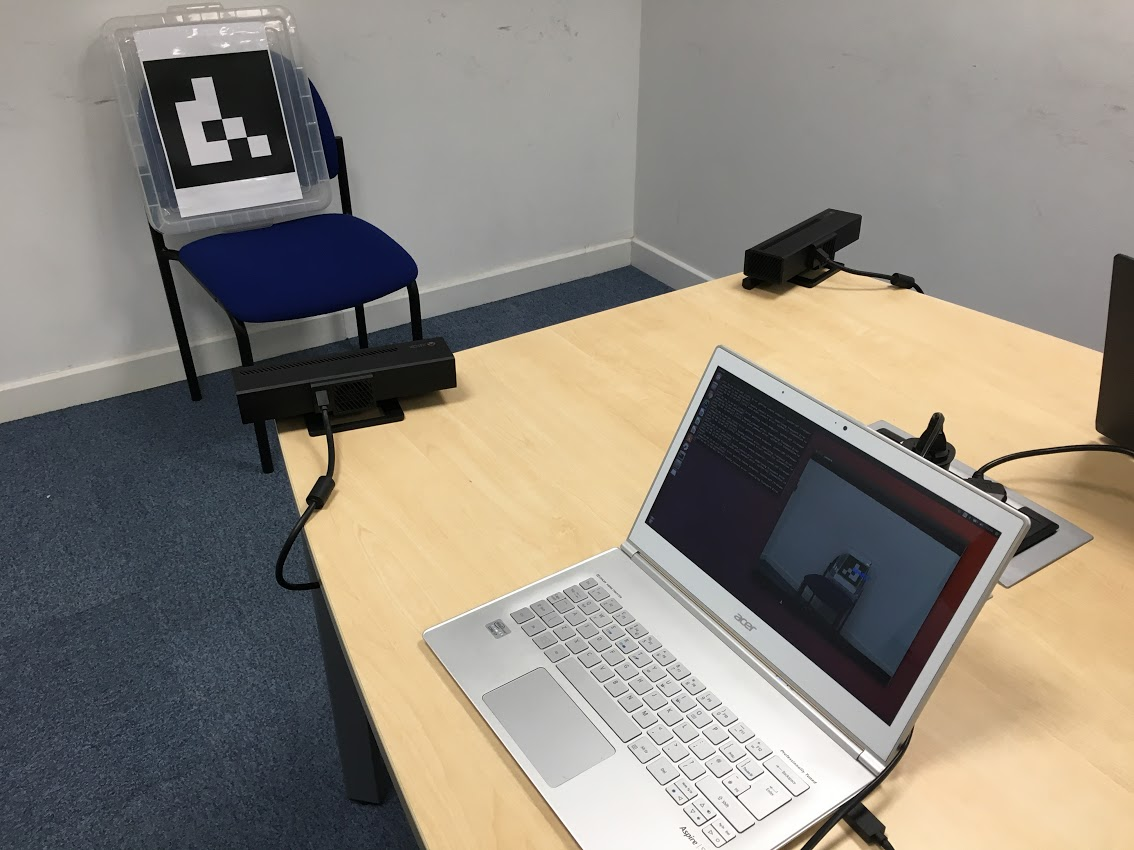
\includegraphics[scale=0.175]{pointifysetup}
\end{subfigure}
\begin{subfigure}[b]{0.49\textwidth}
  \centering
  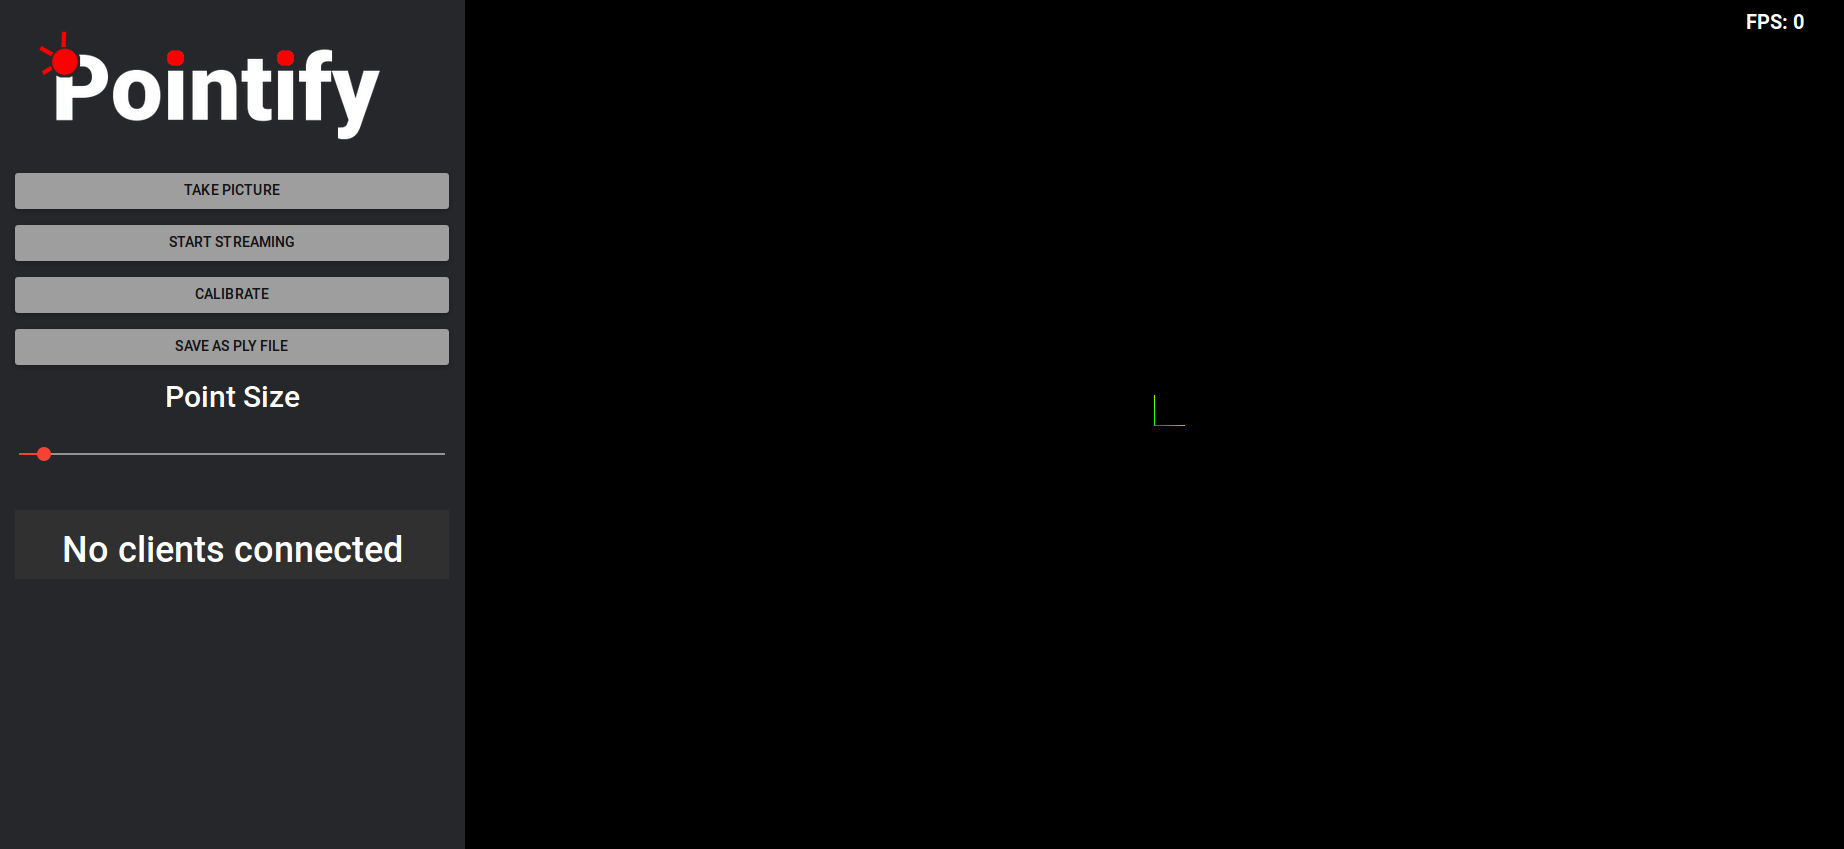
\includegraphics[scale=0.15]{pointifyserver}
\end{subfigure}
\caption{Client and server setup of the \texttt{Pointify} system}
\label{fig:pointifydemo}
\end{figure}

\subsection{Background and Motivation}
A point cloud is a set of points in some coordinate system, that when viewed together form a three-dimensional scene. These structures can be applied to many fields, for example creating three-dimensional models for virtual reality games, manufacturing, 3D printing and medical applications. Gathering the points is done using one or more 3D imaging devices, calibrated with each other. Microsoft \texttt{Kinect V2} is one such device which is widely available and affordable, and includes both a depth and colour sensor as required making it a suitable device to use in this situation. In theory any device with both a depth and colour sensor could be used.
\\\\
We designed \texttt{Pointify} to be an application that makes use of multiple sensors to easily create aligned point clouds by calibrating and combining the input from them. \texttt{Pointify} provides a web interface to view and explore these 3D scenes, as well as export them to use in other applications in a way that is intuitive to use, and easily configurable.

\subsection{LiveScan3D}
The initial goal of our project was to improve an existing open source application called \texttt{LiveScan3D} \cite{livescan}, a research project that has similar functionality to \texttt{Pointify}. Our supervisor, Ben Glocker, proposed that we could improve the calibration step in \texttt{LiveScan3D} \cite{livescan}. At that time \texttt{LiveScan3D} \cite{livescan} was using its own implementation of marker detection and pose estimation, and it was not making use of the open source libraries like \texttt{ArUco} \cite{aruco} or \texttt{OpenCV} \cite{opencv}. \texttt{LiveScan3D} \cite{livescan} is only available on Windows machines and must be compiled using \texttt{Visual Studio} \cite{vs}. The fact that it is not designed to be cross-platform resulted in quite a few difficulties relating to project management, as well as being a limitation on the usefulness of the final product. Furthermore, we found that the code was lacking proper software engineering practices and documentation. We spent 2 weeks trying to make progress with the project, but eventually we decided to pivot and proposed to implement our own version that would be cross platform, as well as incorporating \texttt{OpenCV} \cite{opencv} and \texttt{ArUco} \cite{aruco}. This would make the application more flexible for the users as well as making the product more extensible for developers who may choose to work on different platforms. By approaching it from a software engineering standpoint rather than a research one, we ensured that our code was readable, extensible, and used industry-standard, cross-platform drivers, libraries and frameworks.
\begin{figure}[h]
\centering
\begin{subfigure}{.49\textwidth}
  \centering
  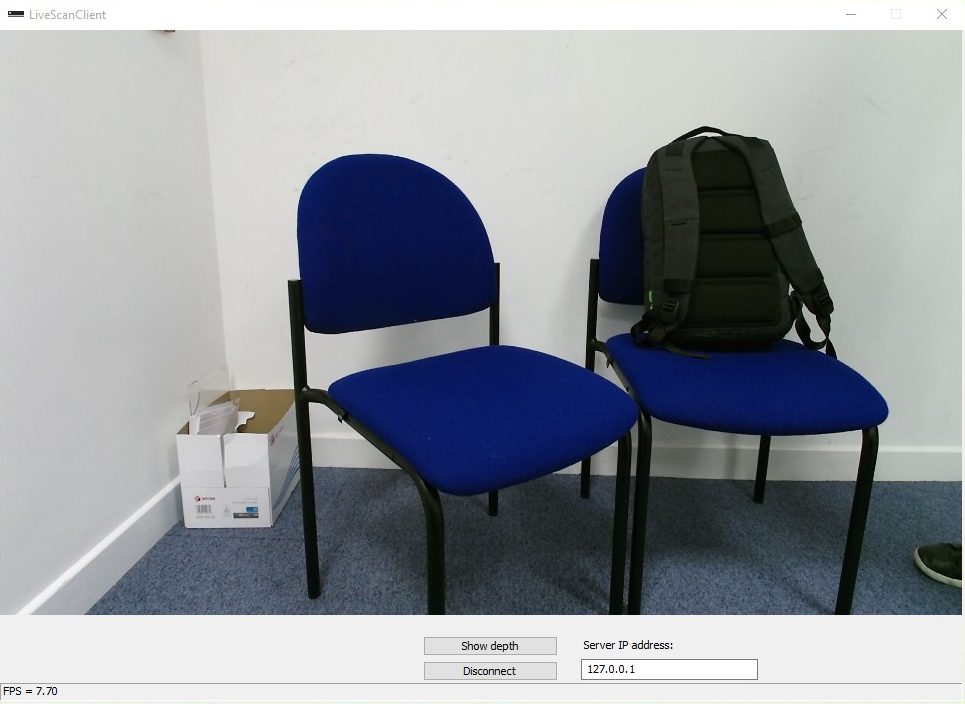
\includegraphics[scale=0.4]{livescanclient}
\end{subfigure}
\begin{subfigure}{.49\textwidth}
  \centering
  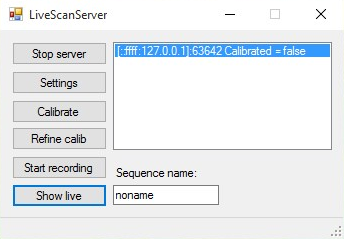
\includegraphics[scale=1.2]{livescanserver}
\end{subfigure}
  \caption{Screenshots of \texttt{LiveScan3D} \cite{livescan} being run with a single \texttt{Kinect} camera}
  \label{fig:livescan}
\end{figure}

\newpage
\subsection{Objectives}
The first two weeks that we spent working on \texttt{LiveScan3D} \cite{livescan} gave us a clear understanding of what purpose our application should serve and how we can achieve that. We decided to follow \texttt{LiveScan3D}'s \cite{livescan} client-server model with multiple clients sending fragments of the scene to a server, which would display them in the same coordinate system to the user. We aimed for a more flexible way of displaying the data, so we chose to use a web application to act as a front end, as it can be accessed on any device with a web browser.
\\\\
The initial aim of the project was to:
\begin{itemize}
  \item Build a distributed system that can gather and merge point cloud data from multiple \texttt{Kinect V2} cameras
  \item Stream the three-dimensional scene to viewers in real-time
  \item Be able to display the point clouds in a way that is convenient for the user
  \item Use standard libraries and frameworks, making the code easy to understand and robust
  \item Ensure that the project is cross-platform (Windows, Linux, OS X)
  \item Allow for the set up and calibration of the cameras to be simple
\end{itemize}

\subsection{Achievements}
After the final iteration of the project, we evaluated our system and what it achieved, and which of the project objectives were completed:
\begin{itemize}
  \item Distributed system consisting of multiple clients with \texttt{Kinect V2} cameras, a server and a viewer allowing the user to easily control the \texttt{Kinect V2} clients and generate the point clouds
  \item Rendering generated point clouds with low latency 3D video streaming
  \item Usage of cross-platform frameworks and drivers allowing the project to be run on Windows, Linux and OS X operating systems
  \item Exporting the data in the \texttt{PLY} format
  \item A simple calibration process that can be done in seconds
\end{itemize}

\newpage
\section{Project Management}
\subsection{Project Plan}
Before we started looking into the specific requirements of this project, we met to discuss how we would proceed with designing and integrating our code, planning how we would use project management tools and software engineering techniques. We set out the following two week rolling iteration plan:

\subsubsection{Iteration One}
We spent the first iteration reviewing \texttt{LiveScan3D} \cite{livescan}, familiarising ourselves with the problem and the libraries we would use to solve it. We dedicated a whole iteration to this, as we wanted to have a strong understanding of the problem before starting work on our solution, as well as have a chance to gather information on the tools we could use to solve it. 
\subsubsection{Iteration Two}
We planned to start building our solution in the second iteration, specifically building a client application that could read from the \texttt{Kinect V2} cameras and display the output. We also needed a web application to display a point cloud to the user, as well as controls to take pictures or start streaming data. We planned to set up our project management techniques and required libraries at the start of this iteration, so they would be ready to use when we started implementing our solution.
\subsubsection{Iteration Three}
We aimed to be able to send a static point cloud from a single camera to the viewer in the third iteration. This involved converting the data captured from the sensor into a format we could send across the network, and decoding this before displaying it to the user. We anticipated that the setting up of the network components would be troublesome, and we would need some time to experiment with different ways of sending the data, in order to find an efficient method.
\subsubsection{Iteration Four}
In the fourth iteration we aimed to implement calibration, allowing us to connect multiple sensors and stream their captured data to the server simultaneously, with the point clouds they capture aligning. This would involve working with the \texttt{AruCo} \cite{aruco} library, as well as combining input from multiple sensors together to give us a a view of many point clouds aligning.
\subsubsection{Iteration Five}
We planned to dedicate the final iteration to bug fixing and optimisation. There was a high chance that our final solution would have inefficiencies, so we planned to spend a significant amount of time fixing these as the application is performance critical. We wanted to ensure that we could stream the scene at a good frame rate with little to no errors or crashes. This was also a chance to add any small features we had thought of during implementation, as well as clean up the code and work on the user interfaces.

\newpage
\subsection{Management techniques}
\subsubsection{Version Control}
When working in a team this size, some form of version control is essential. We chose to use git, hosted on \texttt{GitHub} (https://github.com/jacekburys/pointify) because of our team's familiarity with the platform. We tried to follow the \texttt{Git Flow} \cite{gitflow} branching model, as our project involved adding many features, one at a time, so following the "branch per feature" practice seemed logical. We mainly worked on our own separate branches, merging to master before a checkpoint, or when an important feature was complete and working. 
\begin{figure}[h]
  \centering
  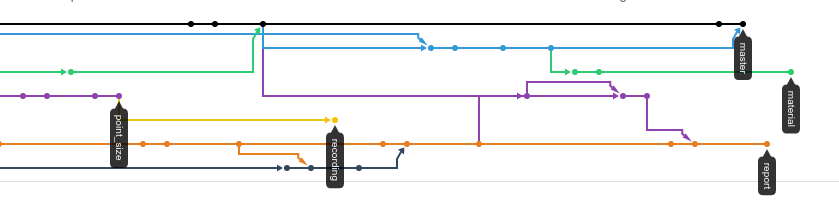
\includegraphics[scale=0.5]{github}
  \caption{Branch techniques from GitHub}
  \label{fig:github}
\end{figure}
\\
\subsubsection{Task Board}
We found a \texttt{Kanban}-style board \cite{kanban} very useful to help us manage tasks throughout the project. We chose to use a web platform called \texttt{Trello} \cite{trello} for this, as it allowed for all team members to view and edit the board anywhere, as well as providing all the tools we were looking for. We classified each task in to three lists, one labeled "Queued" for tasks that have been planned but not started, then "In progress" for tasks that are currently being worked on, and a list for tasks that had been finished, called "Complete". We would assign these tasks to team members during our meetings, then update the status of the task as we worked on it. We aimed to keep the amount of "In progress" tasks as low as possible, focusing on finishing tasks that were semi-completed before moving on to something new. \texttt{Trello} \cite{trello} would automatically notify team members when their tasks had been updated, which allowed us to effectively stay updated with the state of the project between meetings. 
\begin{figure}[h]
  \centering
  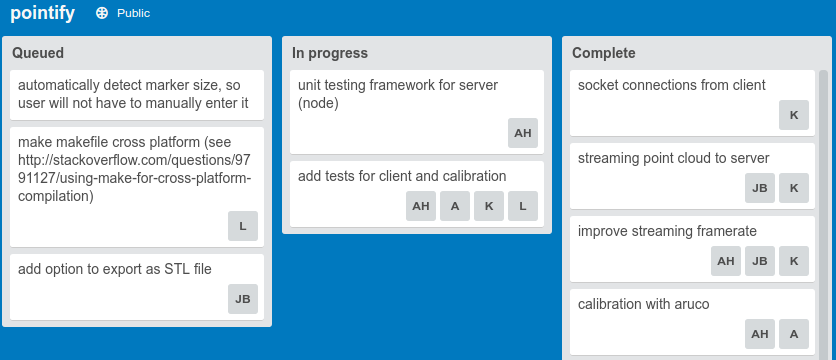
\includegraphics[scale=0.5]{trello}
  \caption{\texttt{Trello} \cite{trello} project management board}
  \label{fig:trello}
\end{figure}
\\
\subsubsection{Continuous Integration and Deployment}
As our project involved building a client-server style system, we wanted somewhere that was able to persistently run the server to help when developing and demonstrating the tool. We used the Department of Computing's \texttt{CloudStack} \cite{cloudstack} instance for this, because of it's easy availability and powerful resources. 
\begin{figure}[h]
  \centering
  \includegraphics[scale=0.25]{cloudstack}
  \caption{\texttt{CloudStack} \cite{cloudstack} instance}
  \label{fig:cloudstack}
\end{figure}
\\
We wanted to spend as little time as possible manually running automated tests and following deployment processes, so we decided to use a continuous integration and deployment tool to automate this for us. We chose \texttt{TeamCity} \cite{teamcity} as our tool, as it integrated well with our \texttt{GitHub} repository, and would run in the background of our deployment server. \texttt{TeamCity} \cite{teamcity} would listen for pushes to the master branch of the \texttt{GitHub} repository, then try to build the code and run all automated tests over it. If all these steps were successful, and all the tests passed, we would push the changes to the deployment instance, which would be available to anyone in the college. This proved to be very useful when a single member was testing the functionality of the client software, as it required a connection to the server to run, so having a persistent instance of the server available at all times was essential. 
\begin{figure}[h]
  \centering
  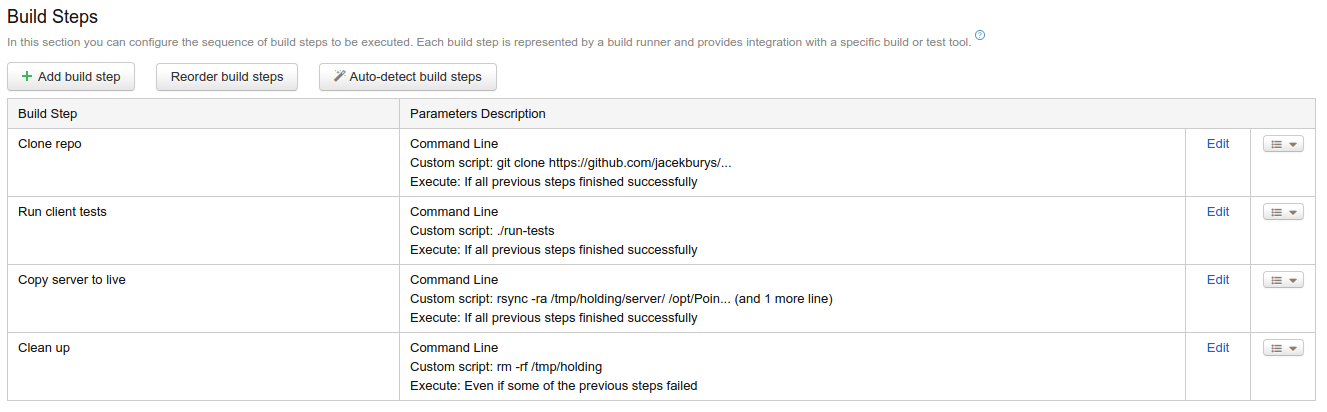
\includegraphics[scale=0.35]{buildserver}
  \caption{\texttt{TeamCity} \cite{teamcity} build and deployment process}
  \label{fig:buildserver}
\end{figure}
\\ 
\subsection{Team Meetings}
As our project involved a lot of interaction between different parts of the code base, we had to meet often in order to discuss how this would work. We aimed to hold formal group meetings weekly, to update the team on our progress and allocate tasks for the next week, as well as meet with our supervisor to demonstrate our progress and listen to his advice. The meetings helped us keep track of what each team member was doing, as well as giving us insight into when specific parts of the project would be completed. We also held more frequent meetings during the week to discuss specific tasks that needed collaboration and sometimes work on important features together in a pair programming environment to ensure their quality. 
\subsection{Task Allocation}
After we had investigated the task in more detail and understood exactly what was needed of us, we were in a position to allocate tasks to group members inside our \texttt{Trello} \cite{trello} board. The main tasks involved building the client system, the server system, working with the \texttt{ArUco} \cite{aruco} calibration library and ensuring the software could be built cross platform. We informally assigned team members to these tasks, with each member putting most of their focus on to their task. From these general aims, we would break them down into more specific tasks, such as "Improve front-end playback frame rate". We tried to write our tasks such that each of them would give a real benefit to the end user, and improve their experience with the product.
\begin{figure}[h]
  \centering
  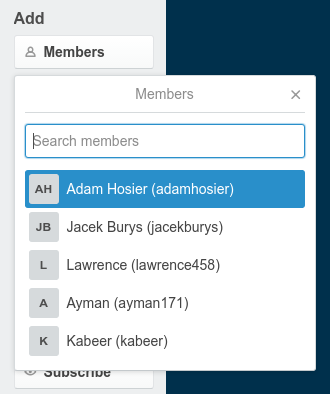
\includegraphics[scale=0.5]{trello2}
  \caption{\texttt{Trello} \cite{trello} task allocation}
  \label{fig:trelloTasks}
\end{figure}

\newpage
\subsection{Issues}
\subsubsection{LiveScan3D}
\texttt{LiveScan3D} \cite{livescan} is run solely on Windows and uses \texttt{Visual Studio} \cite{vs} with Microsoft \texttt{Kinect SDK 2.0} \cite{kinect}. This posed us many problems as a group because only 3 of the members of the group used Windows systems. We also had a problem that with one of the computers, the version of Windows was the 'N' edition of the operating system. Although we tried the recommended fixes on the internet, we were unable to get \texttt{LiveScan} to run on this version of Windows due to errors about missing \texttt{MSVCP120.dll} and \texttt{MFPlat.dll}. This meant that only 2 machines were able to run the \texttt{LiveScan} software which meant there was only one client and one server running. This did not allow us to test the feature of multiple calibrated cameras and also hindered our development since we were only able to work on 2  computers.
\\\\
We also found it difficult to work with the code-base provided by \texttt{LiveScan} as the quality of the code was poor and did not utilise \texttt{OpenCV} \cite{opencv} for matrix operations nor did it use any of the leading calibration techniques. This resulted in code that was highly fragile and highly coupled which posed us issues when we were trying to perform tasks like replacing the calibration system.
\subsubsection{Pointify}
When we opted to pivot the project and work on \texttt{Pointify}, we were able to alleviate a lot of the issues that we encountered when working with \texttt{LiveScan3D} \cite{livescan}. We did however have issues that we encountered during development. When we initially started development, we needed to start development on a single operating system. We chose to begin development on Linux but this meant that we needed
%to dual boot our computers or run Linux through a virtual machine. <-- doesn't make sense
to use virtual machines. This meant that we were not able to begin development immediately due to the time it took to ensure that our systems were set up correctly. This also posed issues of speed when it came to processing power and networking speeds that were crucial during the development of the system. With virtual machines we were only able to allocate partial amounts of our resources to it, restricting the performance inside the operating system, this was also a problem with networking as the virtual machine uses NAT translation to control the networking within the virtual machine which hindered the network contributing to latency and therefore lag in the streaming. Another problem that we faced with the NAT translation was jitter which caused a delay with each individual packet affecting the obtained frame rate. 
\\\\
There were also hardware issues that we had to deal with. We had designed the system to be able to work with multiple cameras and calibrate them correctly. We however for the project were only provided with two \texttt{Kinect V2} cameras to develop with. For testing with the picture taking, we were able to use the cameras in different positions in order to emulate how the system would be able to deal with multiple cameras. This was a sufficient method to be able to test how the calibration would be able to cope and how the rendering was able to cope with a large volume of points. For live streaming however this proved to be much more difficult. We were unable to test how the system would be able to cope with multiple cameras sending data at once and how this would affect the frame rate. The fact that we needed to use the hardware to test the system was also a problem that we faced which meant that we were only able to work on the project when we were in university rather than being able to do any work remotely. For testing purposes we set the build server to be a persistent server for \texttt{Pointify} as well which allowed us to test the client in isolation without having to use a separate machine to act as the server for our distributed system. We had a problem with USB 3.0 ports as well, some of the computers that we were trying to use did not have USB 3.0 which is required for \texttt{libfreenect2} \cite{libfreenect} drivers to be able to communicate with the camera.
\newpage

\section{Design}
We designed the project as a distributed system which has one server and multiple Kinect clients and one viewer. This architecture would allow for further extensibility of the product if other developers wanted to create other types of clients, which is possible by following our interface.
\iffalse % COMMENT START
We decided to do it like this to allow for further usability in the future if the user decides to use multiple cameras in a space and also to improve the extensibility of the product for potential new developers who may wish to create different types of clients which is possible with a standard interface.
\fi % COMMENT END


\subsection{SocketIO}
We decided to use \texttt{Socket.IO} \cite{socketio} to communicate between the clients and the server as it provides a simple to use interface to the underlying networking code. This allows us to create an abstraction away from the underlying network code as well as allowing a standard interface if in the future alternative clients wish to be developed. \texttt{Socket.IO} \cite{socketio} has a C++ client as well as a JavaScript client which meant that we did not need to consider the networking protocols for dealing with the sockets between the server and the client. When calibrating, the server simply sends a calibration request to the client which then sends back a message informing if the calibration was successful or not. When streaming, the server simply requests a picture from each client every frame and synchronises the received frames itself so that all the client needs to do is implement one function to take a picture and does not need to know whether it is streaming or not. The server also sends notifications to start or stop streaming over \texttt{Socket.IO} \cite{socketio} so that the client can change its state when streaming if required. This is done to aid further extensibility.

\subsection{Distributed System}
We chose to design our system as a distributed system for a few main reasons. Using a distributed system is good for applications like these because when adding more devices to the system, more computers and computing power is being added.
%This means that increased number of cameras has a negligible increase on the load of the server which makes the system more powerful.  << THIS IS WRONG
Another advantage of this design is that the cameras do not need to be physically connected to a single computer and can be situated in different corners of the space. This is a vital feature for some of the use cases of our system, such as imaging a point of interest which would require the cameras to be quite far from each other. However, here are also drawbacks of the distributed approach. Having a computer dedicated to each camera means that the hardware requirements are greater and having the system run over the network means that the frame rate and latency will be worse than having it all run on one server.
\begin{figure}[h]
  \centering
  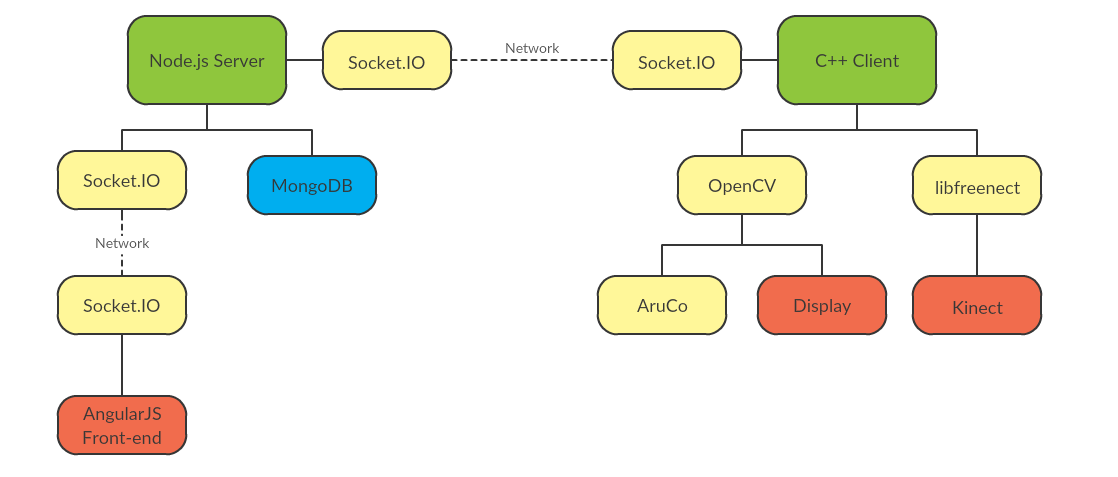
\includegraphics[scale=0.35]{distributed}
  \caption{Diagram of the distributed system design of the project}
\end{figure}
\newpage
\subsection{Kinect Client}
The UML sequence diagram of the client's structure is shown below:
\begin{figure}[h]
  \centering
  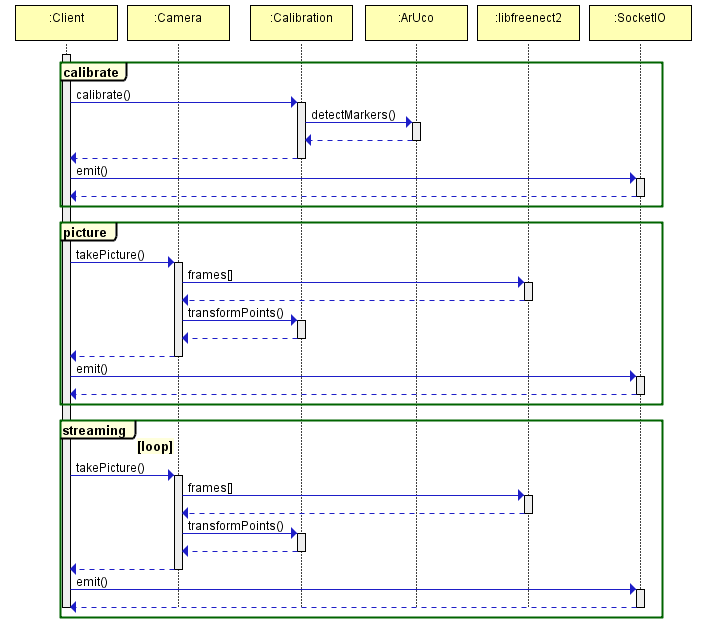
\includegraphics[scale=0.6]{clientUML}
  \caption{UML sequence diagram of the client}
\end{figure}
\\
Each sequence displayed above is triggered by a \texttt{Socket.IO} \cite{socketio} message received from the server. These instructions are received at the client initially. When calibrating, the client takes a frame from \texttt{libfreenect2} \cite{libfreenect} which takes a picture on the camera. It then uses the frame to perform the calibration with \texttt{ArUco} \cite{aruco} which returns rotation and translation vectors, these vectors are then stored within the calibration class. Once this is done, a successful calibration message is sent back to the server. During the take picture, the frame is retrieved in the same way as the calibration and then \texttt{transformPoints} is called which the calibration class uses to transform the points with its internal rotation and translation vectors. It then sends the calibrated point cloud to the server via \texttt{Socket.IO} \cite{socketio}. The streaming function is the same as the take picture except that it happens in a loop. This does not require a separate sequence however as the server deals with the synchronisation and requests the frames when it is needed.
\subsubsection{C++}
We were required to work in C++ for this part of the project in order to make use of the existing libraries that allowed us to interface with the \texttt{Kinect V2} cameras and calibration libraries. C++ is known for it's speed,
%and expressiveness
making it a good fit for this project, as some parts of the client are performance critical. There is a large amount of documentation on C++ and the libraries we were using, making it easy to read up on the methods we were using.
\subsubsection{ArUco}
\texttt{ArUco} \cite{aruco} was the calibration system that was proposed by our supervisor Ben Glocker. It is the current leading calibration system and is provided as a module for \texttt{OpenCV 3.1} \cite{opencv}. Using standard libraries over implementing it ourselves reduces the possibility of bugs and the development cost. Standard libraries also makes our code easier to read for future developers to extend. It is also faster than \texttt{AprilTags} \cite{april}, which is the other calibration system. \texttt{ArUco} \cite{aruco} makes use of different sized markers (see Figure \ref{fig:arucomarker}) when calibrating, we chose 4x4 markers printed on A4 paper to use for calibration, but wanted to be able to tweak this easily.
\begin{figure}[h]
  \centering
  
\includegraphics[scale=0.6]{aruco}
  \caption{Example \texttt{ArUco} \cite{aruco} marker}  
  \label{fig:arucomarker}
\end{figure} 
\subsubsection{OpenCV 3.1}
\texttt{OpenCV} \cite{opencv} is the industry standard open source library for computer vision. It can be used in C++, C, Python and Java for Windows, Linux, OS X, iOS and Android. OpenCV is very optimised for efficiency due to its large developer base and this performance is essential for us since we use it on every loop of our camera to hold the captured images in matrices, and perform operations on them. It can also take advantage of multi-core processing and since almost all devices are multi-core now hence this improves the performance of our application. Since it uses \texttt{OpenCL} \cite{opencl}, it can take advantage of hardware acceleration to compute the matrix operations efficiently. It is also the container library for \texttt{ArUco} \cite{aruco}, giving us one less dependency on our code-base.
\subsubsection{Libfreenect2}
\texttt{Libfreenect2} \cite{libfreenect} was our only option when it came to choosing a cross-platform driver to use for communicating with the \texttt{Kinect V2} camera. Microsoft only supplied the \texttt{Kinect SDK 2.0} \cite{kinect} for Windows. This is not a problem, as it provides all the tools we need for this project, namely getting the depth and colour matrices in \texttt{OpenCV} \cite{opencv} format. It utilises \texttt{OpenGL} \cite{opengl} and \texttt{OpenCL} \cite{opencl} libraries for depth processing. The system also supports up to 5 devices so it allows extensibility in the future if someone wishes to use a single computer to host multiple \texttt{Kinect V2} cameras.
\subsubsection{CMake}
Our tool of choice for building the client was \texttt{CMake} \cite{cmake}, as it is a well established tool for building cross platform applications. \texttt{CMake} \cite{cmake} allowed us to write one make script "\texttt{CMakeLists.txt}", which compiled to a build solution that would run on the user's platform. On Unix systems this would be a \texttt{Makefile}, which allowed to user to use "make" to build the application, and on Windows machines this compiled a \texttt{Visual Studio} \cite{vs} solution which could be built inside the application. We had to make sure that the libraries we used were built for the platform that the client was running on. This could be done by building them from source inside our \texttt{CMake} \cite{cmake} file, or providing the users with precompiled binaries for them. For our needs we found it easier to compile the libraries to the platforms we were using, and downloading them onto the machines we worked on. 
\subsubsection{Data}
We chose to perform the calibration on the client and then send the point clouds directly to the server to allow for distributed computation and speed up the transfer of data. This means that the server is not doing too much work at any one time, as the processing is spread out to the client machines. The task of rendering the point clouds is delegated to the machine viewing it on the web app, which may be different to the server, meaning the CPU and GPU power needed to render the point cloud does not necessarily have to affect the server. 
\subsection{Server}
The UML sequence diagram of the server's structure is shown in the figure below:
\begin{figure}[h]
  \centering
  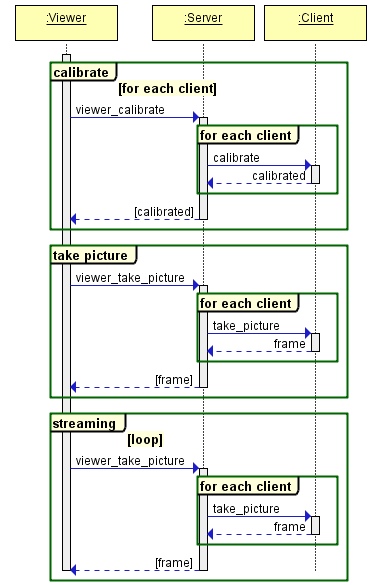
\includegraphics[scale=0.6]{serverUML}
  \caption{UML sequence diagram of the server}
\end{figure}
\\
Each message sent in the diagram above is being sent over the network. During the calibration sequence and the take picture sequence, the viewer sends a single message to the server. The server then sends its message to all connected clients and receives the response that it gets back from each client. It then puts all the responses into an array and transmits the obtained array back to the viewer. This way the viewer is abstracted away from the list of clients. During streaming, the server simply requests pictures from the clients in a loop.
\subsubsection{Gulp}
In order adhere to the good software engineering practices and make the development process more efficient we used \texttt{Gulp} \cite{gulp} which is a toolkit for automating time-consuming tasks that are very often encountered in the process of developing a web-app. It has functionality for linting the code, injecting scripts and CSS files, cleaning the project and many more. All of them contribute to good software engineering design by ensuring that the code is clean and has good style. Thanks to \texttt{Gulp} \cite{gulp} we could start the web-app in a few seconds by running one simple command from the terminal. \texttt{Gulp} \cite{gulp} also allowed us to run a persistent instance of the web-app online, that would update with our GitHub commits without having to reload project files.
\subsubsection{Node.js}
We chose to use \texttt{Node.js} \cite{node} as the framework for building the server. Our plan was that the server would be just aggregating the data from the \texttt{Kinect} clients and sending it to the web app front end. \texttt{Node.js} \cite{node} seemed like a good choice because it is known for its high throughput and we did not plan to do too much CPU intensive processing on the server side. Furthermore, it is currently one of the most popular framework with a large set of available packages.
\subsubsection{AngularJS}
\texttt{AngularJS} \cite{angular} is one of the most popular frameworks for front-end development. It uses \texttt{JavaScript} as its programming language and utilizes the Model-View-Controller architecture, which makes it possible to build interactive and seamlessly working applications. Furthermore, it is relatively easy to use and we had past experience with it, which increased the speed at which we could progress with the web app.
\subsubsection{Angular Material}
A pleasant and easy to understand user interface is a vital part of every web app. There is no need to design the UI components from the scratch, instead, it is more efficient to use one of the available UI frameworks. We begun the project with \texttt{Bootstrap} \cite{bootstrap}, but later decided to switch to \texttt{Angular Material} \cite{material} because it looked better visually and is as easy to use as \texttt{Bootstrap}. Using pre-built UI tools allowed us to focus most of our time on the functionality of the product, as we were aware that designing a good UI is a time consuming task that would not greatly contribute to our project objectives.
\subsubsection{Three.js}
Being able to render the point clouds is essential in \texttt{Pointify}. As none of us had previous experience with
rendering 3D scenes we had to look for a good library that would help us with that. At first we found an open source project called \texttt{Potree} \cite{potree} which is a 3D renderer designed specifically for large point clouds. However, having done more research we came to the conclusion that it would be too advanced for what we actually needed. This would introduce more unnecessary complexity, so we decided to use \texttt{Three.js} instead. \texttt{Three.js} \cite{three} is a \texttt{JavaScript} 3D library which makes it really easy to render 3D scenes in the browser. Fortunately, it supports point clouds and turned out to be perfect for our needs. Both of these solutions run on top of \texttt{WebGL}, the standard framework for graphical applications in web browsers. We were aware that writing a solution from scratch in \texttt{WebGL} would be a challenging task, so chose to use an existing framework to aid us here.
\subsubsection{Bower and npm}
Most of the frameworks and libraries outlined above can be automatically downloaded using \texttt{npm} \cite{npm} or \texttt{Bower} \cite{bower}, therefore we utilised these two package management systems to simplify the installation process. \texttt{npm} \cite{npm} is used for \texttt{Node.js} \cite{node} packages, whereas \texttt{Bower} \cite{bower} manages packages used by the front end.

\newpage
\section{Implementation}
\subsection{Boilerplate generation}
As in most of web development projects, there is a lot of boilerplate code that just has to be written and is very similar in every project. We decided to use \texttt{Yeoman} \cite{yeoman}, which is a scaffolding tool that allows the users to select the frameworks and generates the project structure and a basic template of the web app. We then modified that template by adding our own parts. This saved multiple hours of work.
\subsection{Front end}
\subsubsection{Overview}
We wanted to develop a single command center from which all the Kinect clients would be controlled. Our front end does exactly that. There are two main parts, the controls and the point cloud renderer. We used \texttt{AngularJS} \cite{angular} to control the behaviour of the buttons, which then is passed to the server via \texttt{Socket.IO} \cite{socketio}. When the server sends the point cloud data to the front end, it is then passed to the \texttt{Three.js} \cite{three} renderer which allows the user to view the point cloud.
\subsubsection{Communication with the server}
We chose to use \texttt{Socket.IO} \cite{socketio} as the way of communication between the front end and the server. Each action of the user on the control part of the app sends a \texttt{Socket.IO} \cite{socketio} message to the server. This was simple to implement, following the well documented API that \texttt{Socket.IO} \cite{socketio} provides. 
 % TODO : I don't know what else can be written here
\subsubsection{Point cloud rendering}
Point cloud data is obtained from the server via \texttt{Socket.IO} \cite{socketio} as a single chunk of bytes. This implementation decision allowed us to reduce the amount of data being sent and thus speed up the frame rate. The bytes then have to be parsed and converted into the coordinates and colours of the points. Finally, the data is being passed to \texttt{Three.js} \cite{three} to render.

\subsection{Server}
\subsubsection{Communication with the clients}
Most of the communication is done using \texttt{Socket.IO} \cite{socketio}. We defined a set of messages for the viewer and another set of messages for the \texttt{Kinect V2} clients. On a connection, the server recognizes whether the request comes from the viewer or a \texttt{Kinect V2} client and handles them in different ways. According to our design, we intend only one viewer to be connected at the time, therefore the socket connection from a viewer is saved and used from that point overriding the previous connection. When the connection request comes from the \texttt{Kinect V2} client, it is added to the list of connected clients and receives all control messages from that point onwards and is expected to provide its part of the scene.
\subsubsection{Synchronization}
The \texttt{Kinect V2} clients work independently and produce parts of the whole scene that should almost perfectly overlap when rendered together after calibration with \texttt{ArUco} \cite{aruco}. However, if the object is moving and different parts of its point cloud representation taken at different time, the model will be inaccurate. To minimise this effect we had to come up with a way to synchronize the \texttt{Kinect V2} clients so that the data belonging to one point cloud scene is taken from the sensor at approximately the same time. Our approach is to make the \texttt{Kinect V2} clients generate the point cloud parts continuously and keep the latest one in a variable. The content of this variable is then sent to the server on a socket message requesting the data.
\subsection{Calibration}
\subsubsection{Marker pose estimation}
When obtaining the data with more than one camera, we required the point clouds they send to be aligned such that they can be displayed seamlessly on top of each other, building a 3D representation of the scene. The idea behind this involves applying a transformation to each point in the scene, to bring it from the camera's perspective to some common perspective shared by all the cameras. We discussed two ways of doing this, one of which chooses one of the cameras as the "master" camera, then synchronises the other cameras around it. The alternative method is by centering all of the cameras on a common point, in our case the calibration marker we use. An advantage of using the first method is that one less camera would need to be calibrated, as all of the other cameras would be centered around the master, but this would lead to more complicated code, and more difficult communication between the cameras. The second approach would give more elegant and maintainable code, as each of the cameras performs the same calibration, but sacrificing a small amount of efficiency on one of the cameras. For these reasons, we chose to use the second approach, calibrating all cameras around the marker placed in the scene. 
\\\\
This involved working with a third party library called \texttt{ArUco} \cite{aruco}, which is a well established computer vision library for C++ that helps with the calibration process. In the method we chose, the cameras are all centered around a stationary marker (similar to Figure \ref{fig:arucomarker}) placed in the scene, so we required \texttt{ArUco} \cite{aruco} to detect these markers and calculate the camera's position relative to the marker. The aim is to find the transformation that brings points centered around the camera, into a space with the marker as the origin, then once this is calculated we can apply this transformation to each point cloud to align them. We start this process by detecting any markers visible in the scene, then finding rotation and translation vectors from the camera to this marker, adjusting for intrinsic camera parameters such as focal length and principal point offset. From this we can build up a transformation matrix to combine both the rotation and translation, before inverting it to get the translation from camera to marker as shown in Figure \ref{fig:transformationMatrix}. \\
\begin{figure}[h]
  \[\left(\begin{array}{cccc}
      & | &   & | \\
    - & r & - & t \\ 
      & | &   & | \\
    0 & 0 & 0 & 1
    \end{array}\right)^{-1}\]
  \caption{Transformation matrix, where \textbf{r} is the rotation and \textbf{t} is the translation}
  \label{fig:transformationMatrix}
\end{figure}
\subsubsection{Point cloud transformation}
Once we have found the transformation matrix as in the previous part, we must apply it to each point cloud before they are is sent to the server. Each \texttt{XYZ} point must be extended with a \texttt{1} on the bottom row, so that it can be multiplied correctly with the transformation matrix. We experimented applying the transformation matrix to each point to give the transformed point, but this was causing some performance issues due to the amount of points needed to be transformed at once. A better way of doing this would be to apply the transformation to all points in one operation with a more complex matrix operation, shown in Figure \ref{fig:transformationMatrix}. We used an optimised implementation of this in \texttt{OpenCV} \cite{opencv} called \texttt{perspectiveTransform} to do this efficiently, which when given the set of input points, and the transformation function we calculated earlier, would return the transformed points we needed. When each client calculated the transformation to bring their origin to the marker and applied this transformation to the point clouds captured from the connect so they could be successfully combined such that they would align.\\
\begin{figure}[h]
  \[\left(\begin{array}{cccc}
      & | &   & | \\
    - & r & - & t \\ 
      & | &   & | \\
    0 & 0 & 0 & 1
    \end{array}\right)^{-1}
  \left(\begin{array}{cccc}
    \multirow{3}{*}{\textbf{$p_1$}} & \multirow{3}{*}{\textbf{$p_2$}} & \multirow{3}{*}{\dots} & \multirow{3}{*}{\textbf{$p_n$}} \\
    & & & \\
    & & & \\
    1 & 1 & & 1
    \end{array}\right)\]
  \caption{Transformation matrix as before, applied to each point $p_1$ \dots $p_n$}
  \label{fig:transformationApplication}
\end{figure}

\subsection{Point cloud streaming}
Once we had built the point cloud, the next step was to send the information over a network to the server. We decided to do this by packing all the points into a binary buffer, as there would be no wasted space. This information we needed to send consisted of three 32 bit floats, for \texttt{x} \texttt{y} and \texttt{z} coordinates, as well as three \texttt{8} bit integers for the \texttt{RGB} colour values, giving a total of \texttt{15} bytes per point. There can be up to \texttt{512 x 424} points in space, giving a maximum total buffer size of \texttt{3180KB} per frame. In reality, this number was much smaller, as the sensor cannot pick up points that are too close or far away. We discussed the idea of compressing this buffer to reduce transfer speed, but as our client software was relatively CPU intensive already, we decided to send the uncompressed data instead.

\subsection{Challenges}
\subsubsection{Dual Camera Sensors}
When performing the calibration we noticed that the calibration was slightly off. After doing some research we worked out that this was caused by the offset between the depth and \texttt{RGB} cameras on the \texttt{Kinect} hardware. The reason for this was that we were performing the \texttt{AruCo} \cite{aruco} calibration on the \texttt{RGB} matrix from the colour camera and then we were using the obtained rotation and translation vectors to calibrate the output from the depth camera. This slight offset caused the obtained origin in the coordinate space to be different and then caused the point clouds obtained from the different cameras to not align correctly. This is demonstrated in figure~\ref{fig:rgbdepth} below.
\begin{figure}[h]
  \centering
  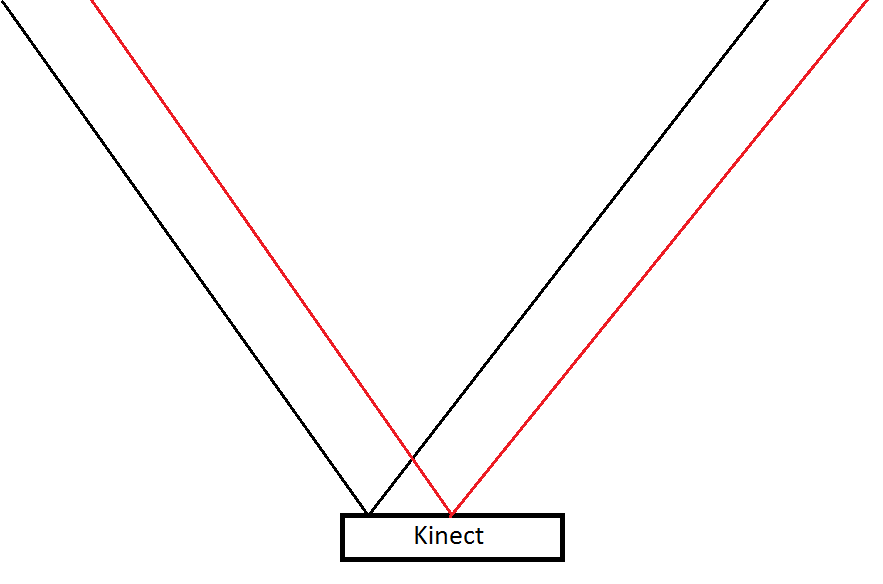
\includegraphics[scale=0.4]{rgbdepth}
  \caption{Showing the offset between the field of view of RGB and depth cameras on the Kinect}
  \label{fig:rgbdepth}
\end{figure}
This produces an offset in the calibration as shown in figure~\ref{fig:calibrationoffset} below.
\\
\begin{figure}[h]
\centering
\begin{subfigure}{.49\textwidth}
  \centering
  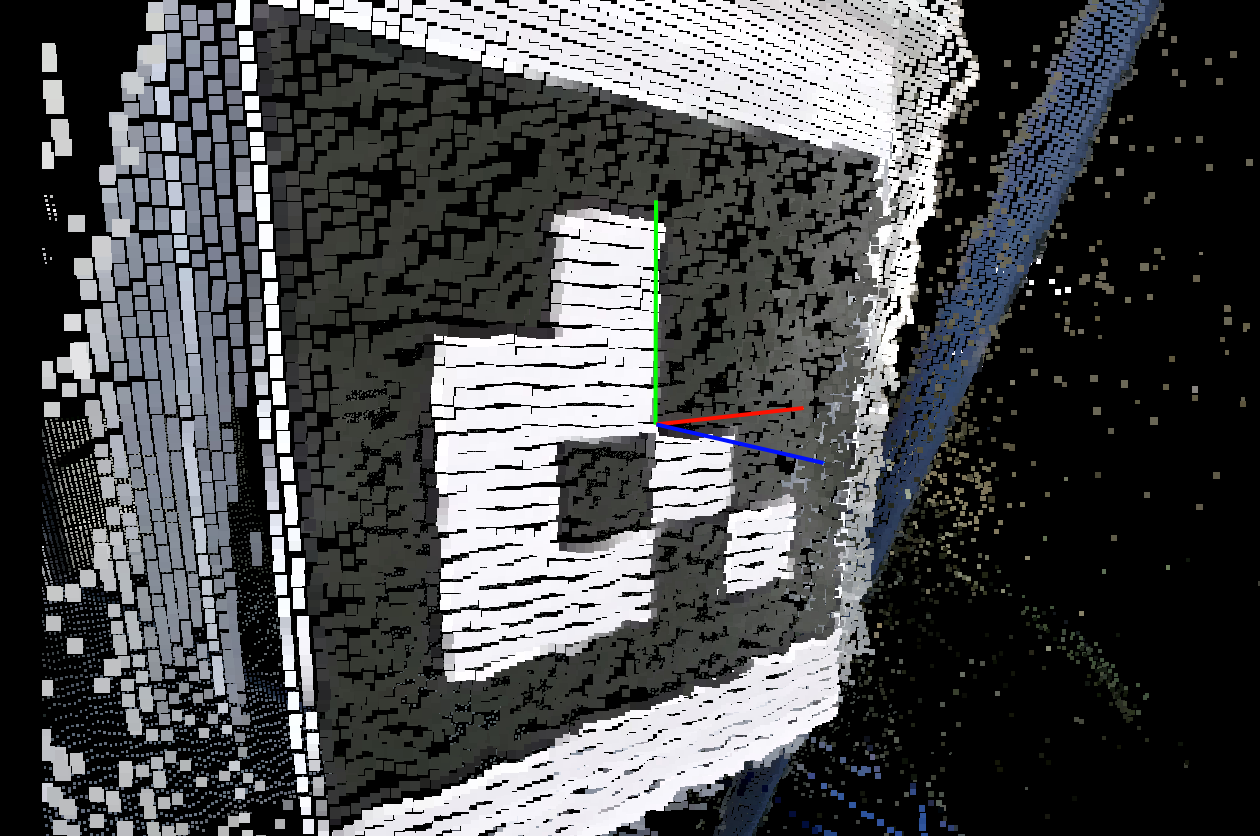
\includegraphics[scale=0.2]{registeredpointcloud}
\end{subfigure}
\begin{subfigure}{.49\textwidth}
  \centering
  \includegraphics[scale=0.2]{unregisteredpointcloud}
\end{subfigure}
  \caption{Showing the offset in calibration with the RGB camera and the depth camera}
  \label{fig:calibrationoffset}
\end{figure}
\\
To fix this issue we needed to use the registered camera matrix from the \texttt{apply} function within \texttt{libfreenect2} \cite{libfreenect}. This gave us a matrix which provided the \texttt{RGB} data points mapped onto the corresponding points from the depth camera's field of view. We therefore performed the calibration from the depth cameras field of view and output the correct resultant rotation and translation vectors for the point cloud generated from this camera.
\newpage
\subsubsection{Calibration Accuracy}
When using the registered matrix, we encountered a much worse camera matrix than the one directly taken from the RGB camera as shown in figure~\ref{fig:registeredaccuracy} below.
\begin{figure}[h]
\centering
\begin{subfigure}{.49\textwidth}
  \centering
  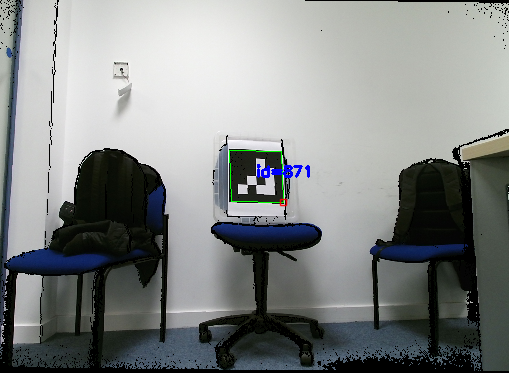
\includegraphics[scale=0.5]{registeredview}
\end{subfigure}
\begin{subfigure}{.49\textwidth}
  \centering
  \includegraphics[scale=0.5]{unregisteredview}
\end{subfigure}
  \caption{Showing the ArUco \cite{aruco} accuracy between the registered and direct RGB matrices}
  \label{fig:registeredaccuracy}
\end{figure}
\\
This reduced quality meant that \texttt{AruCo} \cite{aruco} was unable to as easily detect the markers in the scene, this is a problem we were not able to fully resolve and we have to take it as a limitation of the system. We also noticed that where \texttt{AruCo} \cite{aruco} was unable to detect the marker accurately, there were very small parts of the screen that were being detected as a marker as well as the main marker. This caused us issues as with multiple markers on the screen, when performing the calibration, \texttt{AruCo} \cite{aruco} may choose the wrong marker to calibrate on, causing the points to be calibrated at the wrong location. To rectify this, during the calibration step, if there is more than one marker in the scene we would calculate the size of the 3D planes and then keep only the largest plane and remove the smaller ones. This would then return us with only the main marker in the scene if it was detected correctly.

\subsection{Unsolved Challenges}
There were also a few unsolved challenges that we faced with the project that we have been unable to find a solution to at this time. These challenges that we faced are related to the streaming capability of our system and they are related to the obtainable frame rate of the streaming.
\subsubsection{TCP vs UDP}
With the network we had a major problem with the protocols of TCP vs UDP. Since we are streaming the frames, UDP is a much more desirable protocol to be using to increase the frame rate of our system. The first problem we encountered with using this is that \texttt{Socket.IO} \cite{socketio} only supports TCP communication. We then considered using standard networking protocols rather than \texttt{Socket.IO} \cite{socketio} for the streaming of the frames between the client and the server but we realised that, for the server to communicate between its \texttt{node.js} \cite{node} back-end and its \texttt{Angular.JS} \cite{angular} front-end, it needs to use JavaScript for the rendering of the point clouds. JavaScript as a language does not natively support UDP therefore we realised that even if we would be able to communicate the server and the client, we would encounter a bottleneck between the back-end and the front-end of the server and experience no additional improvement on the frame rate.
\subsubsection{Synchronisation Latency}
High latency is another issue we encountered. We were able to obtain a moderate frame rate between the server and the client for streaming but we experienced on average a 3-second delay between the camera display on the client and the server. We have not encountered any bottlenecks within our system that could be causing this lag and we are assuming that it is simply the network delay that is causing it.
\subsubsection{Socket.IO C++ Client}
The TCP based streaming protocol that \texttt{Socket.IO} \cite{socketio} uses has not been implemented with the current C++ client offered. This meant that during streaming of the frames, we had to send our data via standard \texttt{emit} messages instead. We are not sure as to whether this would have made a significant impact on the frame rate but the data sent over the normal protocol has a much larger header per frame.

\newpage
\section{Evaluation}
\subsection{Design}
We utilised many design patterns when developing the technical structure of our project. For the server we utilised the publish subscribe design pattern for keeping control of the clients that are connected. This model worked well for us as meant that we only needed to design with one client in mind initially and that same design instantly worked with multiple clients as well.
\\\\
We also felt that the client should be kept very simple so we decided to make it a command line tool. Since this project is aimed at technically minded people, we felt that this was a good approach. In the future we may decide to make it a fully graphical user interface to appeal to the general user more.
\\\\
The fact that the server is run as a web application in \texttt{localhost} was a choice that our supervisor Ben Glocker liked from the start and we took inspiration for the idea from \texttt{iPython} \cite{ipython} notebooks which are run in the same way. We feel that the system is easy to use and not overly complicated.
\\\\
The physical design of the server is also minimal. We decided to have all the controls in a navigation pane on the left hand side and then fill the right hand side with the point cloud. This allows the user to have the maximum viewing area for the point cloud and have all the controls intuitively in the sidebar.
\begin{figure}[h]
  \centering
  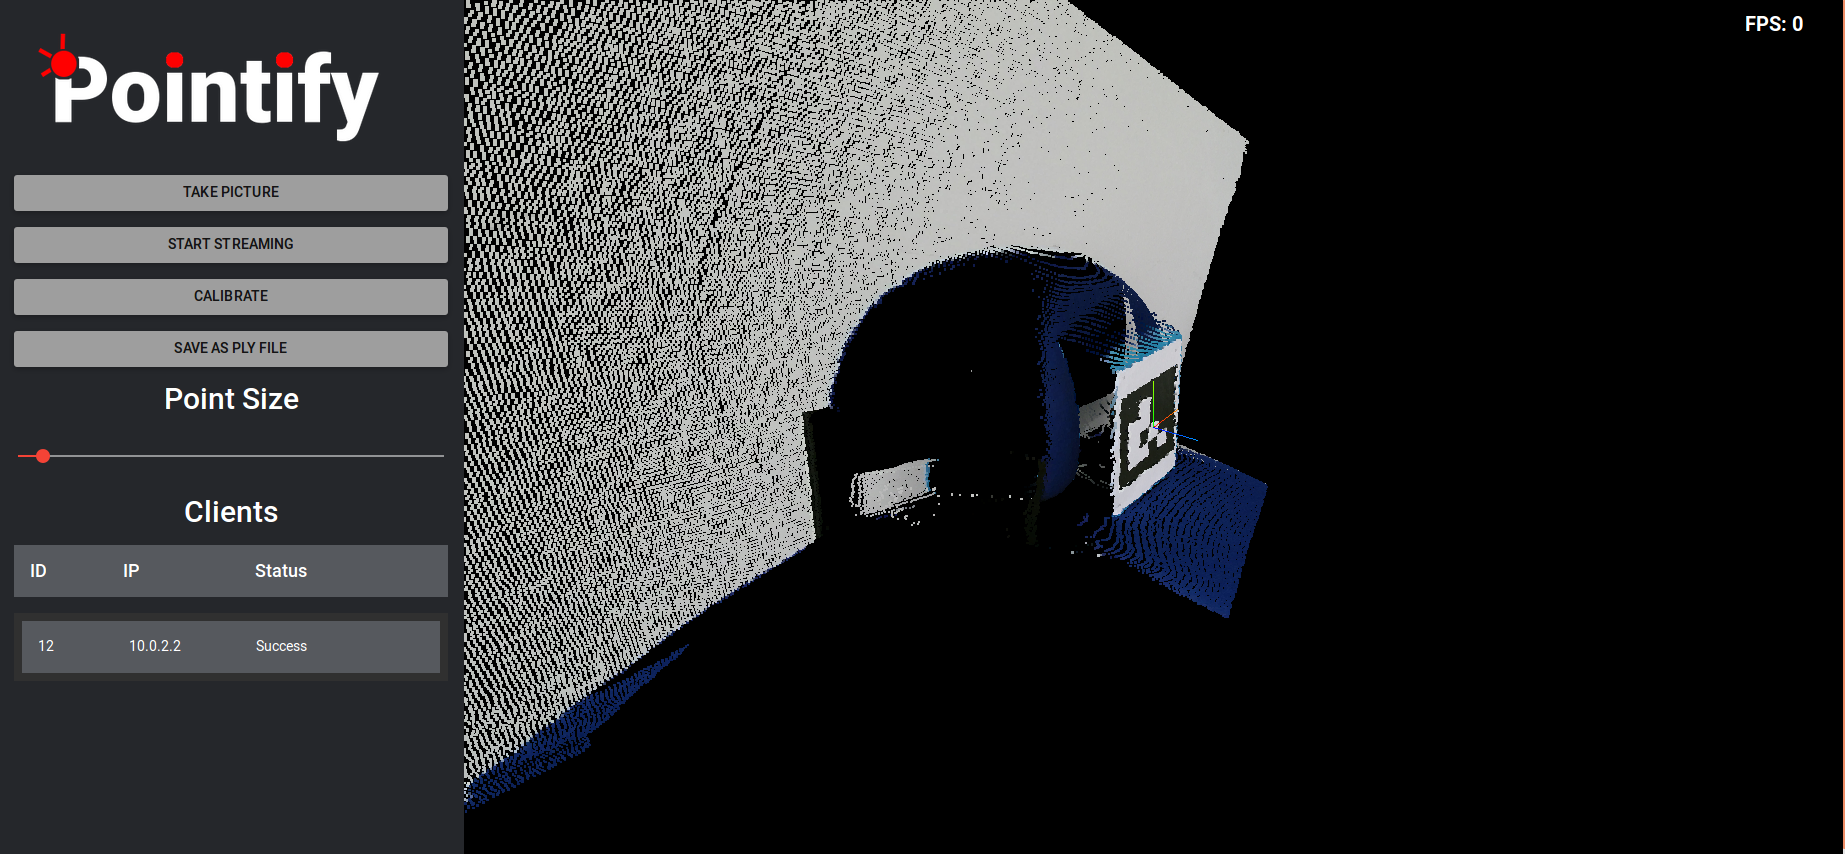
\includegraphics[scale=0.2]{serverdesign}
  \caption{Showing the final design of the server}
\end{figure}
\subsection{Code Quality}
Overall we are fairly happy with the quality of the code we have produced. We approached the code in an object oriented fashion and we have clear communication between the various components of our code. One benefit of the amount of pair programming we did is the peer evaluation of the code as you type which holds the standard to a higher level. We also did not experience more bugs appearing as we progressed throughout the project or did we experience a vastly increased development cost which are indications of low fragility and low rigidity. We also agreed a level of code quality at the start that has been adhered to throughout the project.
\\\\
We utilised branches effectively for each feature of the product so that we could then be comfortable about the quality of any code on a separate branch and the fact that it is working correctly before merging into the master branch. This way we know that the master branch is the release branch of everything that is fully working and if there are issues on other branches we can use the master branch to test with slightly older versions of the code.
\\\\
If we had more time and were pursuing a slower but higher quality level of development we would have done more peer reviewing of each commit before accepting it. We decided not to waste time doing this due to the agile development structure of the project and the fact that we had to have an extensive set of features for the presentation.

\subsection{Calibration Accuracy}
As discussed earlier in the project, the calibration accuracy was a topic that had to undergo certain levels of compromise in order to get it fully working.
\\\\
One of the major causes of issues with \texttt{ArUco} \cite{aruco} was the fact that we had to calibrate on the registered matrix rather than the direct camera matrix. This was much less reliable and we often had issues of the marker not being detected at all even though it was in the scene. We managed to eliminate the issues with \texttt{ArUco} \cite{aruco} detecting ghost markers in the scene but we still suffered with the basic detection of the marker.
\\\\
We tried to improve this by reducing some of the control factors within the scene. We tried to make the marker bigger by maximising the space on the A4 sheet of paper that the marker could occupy. We stuck the marker onto a flat object so that we could eliminate the curve in the marker that we noticed caused a significant decrease in the accuracy of the calibration. We then tried to use different printers for the marker as we noticed that the printers supplied at university used a shiny ink and light which was shining directly on the marker which caused parts of the marker to be blanked out with respect to the camera which caused it to not be detected. We also then tried to make the marker much bigger using an A3 sheet of paper.
\\\\
We noticed that surprisingly, after much testing, the smaller marker was actually able to be detected more easily but the bigger marker provided a more accurate calibrated origin, we decided in the end to go for the full A4 sheet as our marker. We were not extremely satisfied with the quality but we feel that with the time we have available and the restrictions on the hardware, this is the best that we could achieve. We also feel that if we were using a camera where the depth sensor and the camera are close enough to each other that the field of view would not be different, then we would be able to obtain a much higher quality of calibration.
\\\\
Once we had \texttt{ArUco} \cite{aruco} detect the marker in the scene and calibrate successfully, we noticed that the rotation and translation vectors that we were able to obtain were accurate. We were able to stream and take pictures with multiple cameras and have the point clouds align almost seamlessly. We feel that the calibration is extremely fast and also if the right conditions are provided, then the marker can be detected fairly well. We realise that we will not always have optimal conditions for some of our use cases and this is something that we would have to look at for further work.
\\
\begin{figure}[h]
  \centering
  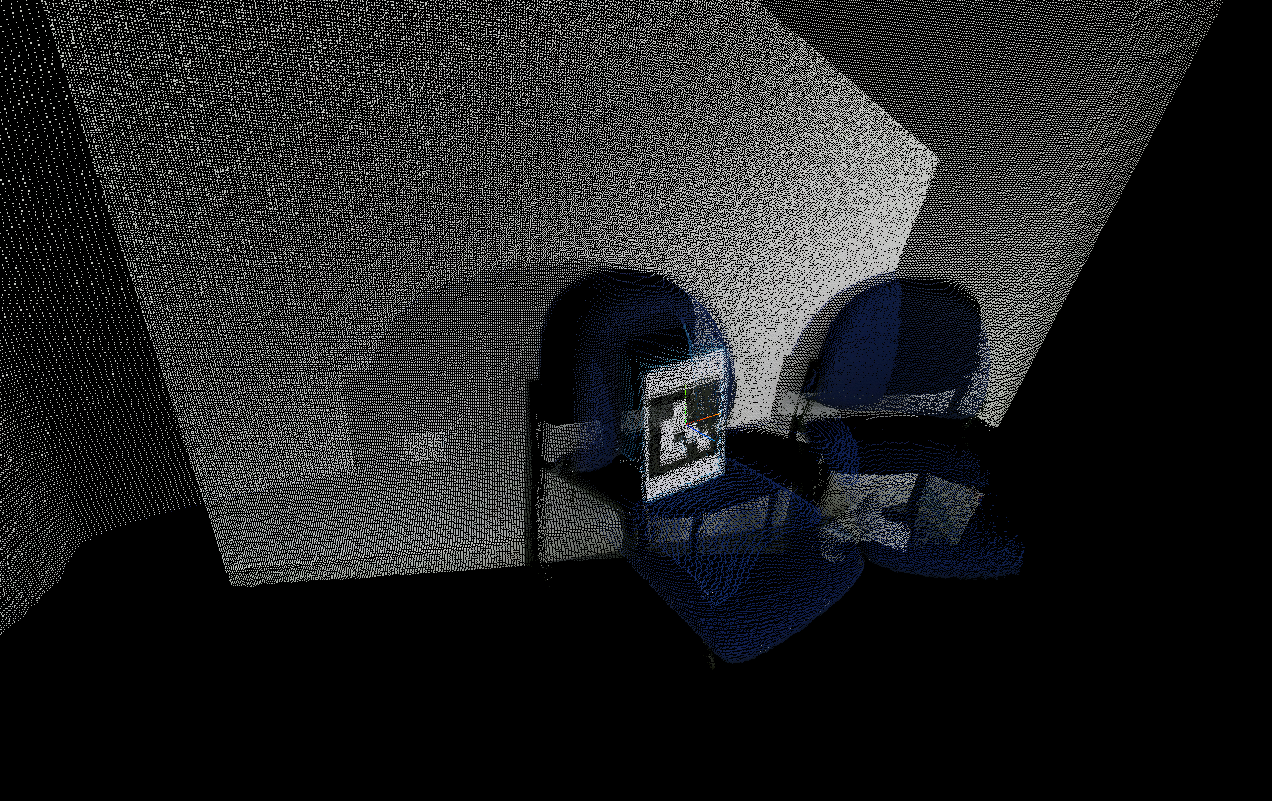
\includegraphics[scale=0.3]{mergedpointclouds}
  \caption{Showing the result of two merged point clouds from two calibrated cameras}
\end{figure}
\subsection{Performance}
Both the client and the server seemed to run well on all of the systems we tested on. There were certain aspects of both that caused the running performance to be affected.
\\\\
In the client we had a loop that was constantly running until the application was closed. It was also registered to many callbacks in \texttt{Socket.IO} \cite{socketio} that it was listening on the entire time. In the main loop of the client we were obtaining the latest frame from the \texttt{Kinect V2} camera and simply displaying it for the user to see using the \texttt{OpenCV} \cite{opencv} \texttt{imshow}. This created a live view of the camera for the user of the client to see when it was running. With the \texttt{ArUco} \cite{aruco} calibration we also decided to add some elements of the calibration to each loop of the camera which affected the performance. We wanted to display a bounding box whenever a marker was detected and send live updates on how many markers there are in the scene back to the server. Both these things negatively affected the client but we feel that the speed is still fairly fast and the improvement in usability is worth the cost.
\\\\
For the server, there are very few elements that happen in real-time when it is not streaming that are different from a standard web application. The server has a front end which dynamically updates whenever the server sends it a message over \texttt{Socket.IO} \cite{socketio}. We use \texttt{Three.js} \cite{three} to render the points which is a very lightweight framework. Apart from the rendering, the server has buttons which send \texttt{Socket.IO} \cite{socketio} messages but there is not much else that runs constantly when idle. Therefore the server is just as fast as any other web interface and perfectly usable.
\\\\
Overall we feel that the performance of the server and the client are
%perfectly
fast enough and we have not experienced any noticeable decrease with any of our systems.

\subsection{Build Server}
The build server helped us massively in the process of testing and running demos. It allowed us to have a persistent instance of the server code live and accessable at all times, allowing a single programmer to work on the client code and test it against the server code. It would seamlessly update whenever a commit was pushed to the master branch, run build checks and unit tests before deploying the code live. Any of us could log in to the \texttt{TeamCity} \cite{teamcity} instance to check the build status and manually run tests, allowing us to be updated with the status of the project easily.
\\\\
A downside of the setup we used is that it was set up to only observe the master branch, which was only updated for major milestones. There were times where we would have liked the server to be observing another branch that was more often updated to test against. Another issue with our setup was how we used the departments \texttt{Cloudstack} \cite{cloudstack} setup, which is only accessable from within college. This meant that whenever we wanted to access the build server from outside of college, we had to take a more convoluted approach, such as using the college VPN.

\subsection{Testing}
We had set up formal test procedures to run before deploying the code live. This involved the \texttt{Catch} \cite{catch} test-suite for C++ and tests integrated to \texttt{Gulp} \cite{gulp} for the server. Due to the nature of the project, testing individual components was difficult, so we relied more on whole system testing to validate if our product was functioning correctly. For example, when testing the calibration, there was no easy way to check if our methods were giving the desired results without manually observing the alignment of the point cloud. 
\\\\
In evaluation, it may have been better to use a more test driven development approach to the project, especially when testing algorithms such as the point cloud buffer packing, as these are easily testable. But there are certain parts of this project which would be extremely difficult to test formally and our manual approach was sufficient. 

\subsection{Deployment}
\texttt{Pointify} is very simple to set up, as intended at the start of the project. The web app can be installed and run easily with just one terminal command thanks to the automation provided by \texttt{npm} \cite{npm}, \texttt{bower} \cite{bower} and \texttt{gulp} \cite{gulp}. The \texttt{Kinect V2} clients can be compiled in the same way on every platform using \texttt{CMake} \cite{cmake}, then run as a standard application from the command line. We think this contributes to fulfillment of the goal for simplicity of use, however the \texttt{Kinect} clients could be difficult to compile for non-technical users. 

\subsection{Streaming}
The streaming was the section we spent most of the time improving towards the end of the project. This was a challenge since we are trying to process, send and render multiple point clouds per second over the network. We found this part the most difficult to test effectively as the load on the network was such a large factor that we would often experience false positives as to whether a certain improvement we had implemented had improved or worsened the obtained frame rate. To negate these issues, towards the end of the project, we opted to create a local network to remove this control variable from our testing. We also used \texttt{LiveScan3D} \cite{livescan} to compare to what frame rate we should theoretically be able to achieve with their systems and what we were achieving, all the while taking into account the extra overhead we had with respect to \texttt{LiveScan3D} \cite{livescan}.
\\\\
One of the first things we attempted to reduce the overhead is to reduce the size of the data being sent. When sending individual points over \texttt{Socket.IO} \cite{socketio}, we were trying to send each point in its own separate message. We discovered after looking into \texttt{Socket.IO} \cite{socketio} that we were not utilising all available space in each message that was being sent and we were sending extra blank bits over the network. To solve this problem we decided to pack all of the points into a string buffer for each frame and send the entire frame as one string message. We found that this considerably improved the frame rate that we were experiencing. The second improvement that we made is that we tried to pre-cache the frame in the client during streaming so that when a new frame was requested, the client did not need to process the frame, it could simply send the latest processed frame immediately. We found that this had a slight improvement on the streaming but also had a slight negative impact on the speed of the client as it needed to perform more computation in each loop. The third improvement that we made was to try and request a frame every time the server had finished processing the frame which would avoid the network getting flooded. We realised with this approach that it actually significantly slowed down the frame rate since the processing time of each frame was more of a cost than the network being flooded. We decided to implement the first 3 changes and we feel this is sufficient for this stage of the project.
\\\\
We also noticed that we were experiencing a considerable amount of lag between when something happened in the client and when it was to be displayed on the server. We also noticed that this lag was getting worse as the streaming duration increased. This immediately gave us the impression that there was a queue somewhere within the system that was holding the frames that needed to be processed and this queue was getting larger because the frames were being produced faster than they were being rendered. To rectify this we decided to store the latest received frame for each camera in the server and only process the one that we have stored on each iteration of the renderer. This worked well in keeping the lag to be consistent during the streaming and not increasing. We did find however that there was still a constant level of lag that we experienced of around 3 seconds which we were unable to reduce further. Hopefully in the future we would be able to come up with a better way of reducing lag that could work better.
\\\\
Another problem we encountered with the streaming was the time synchronisation of multiple cameras within the scene. What we found is that when we were testing with different computers that all had different hardware specifications that one of the clients would be considerably faster than the other and the two point clouds in the same frame would be showing data at different points in time. To rectify this, we decided to make the server only request a new frame from each client once all of the clients had sent their frame. We were not concerned about the clients not sending their frame because if a client disconnects then it is removed from the client pool and the server will not wait for it. We found that this worked well and we were able to keep all of the frames in a time sync. The main problem we found with this was that we would have to wait for the slowest client for each frame. This meant that the streaming was now as slow as its slowest member. We feel that this is sufficient for the current state of the system but we would probably like to implement some more sophisticated synchronisation systems if we were to have more time in the future.
\\\\
Overall we found that the streaming was the hardest section to improve on and after dedicating a considerable amount of time to improving it, we feel that this is the most improvement that we were able to achieve. When working on it in the future we think this is the biggest candidate for improvement.
\newpage
\section{Conclusion and Future Extensions}

\iffalse % THIS WHOLE SECTION IS USELESS
%Ayman, you are useless
\subsection{Conclusion}
When we received the proposal for 3D reconstruction, we were excited to develop the application despite most of our members having very little experience in Computer Vision. It was applicable because a few members of the group were taking the course which allowed them to use the techniques taught and practically apply them in the creation of \texttt{Pointify}. Background research into 3D reconstruction gave us a general idea of what we were aiming to create as we did not fully understand the concept of 3D reconstruction. From the start, ensuring software development practices such as pair programming were maintained throughout the project was one of the primary importances as members were able to discuss their problems together and discuss how they could better implement a solution.
\\\\
The technical aspect of creating \texttt{Pointify} (coming from the idea that an object or a scene can be reconstructed by rendering many points together from captured depth and colour information) took the most time during the 3 months. During this short time we have endured and have managed to produce a stable application, that combined various technologies together to successfully capture depth information through multiple \texttt{Kinect} cameras, perform calibration and then render the many points together to 3D reconstruct a scene. In order to start we had to understand how \texttt{LiveScan3D} \cite{livescan} worked which took some time as we felt that \texttt{LiveScan3D} \cite{livescan} code was poorly structured. However after analysing \texttt{LiveScan3D} \cite{livescan} implementation, several methods were proposed through our group meeting and then a final concrete solution was decided. We then were able to carefully plan out the major sections of the project to which each group member was assigned a task.
\\\\
For some members of the group, it was their first time to use \texttt{Angular.JS} \cite{angular} and \texttt{node.js} \cite{node} so they were able to acquire a new skill as they used it for developing the front and back-end. Although the main focus of the project was ensuring that we completed implementing the features at each iteration, the latter part of the project was spent on debugging and trying to increase the current frame rate from streaming point clouds. To increase the frame rate we tried to stream the point clouds by connecting the server and client through an Ethernet hub rather than WiFi however this only a small increase in the frame rate. Nevertheless, the small increase in the frame rate was noticeable enough. 
\\\\
Given the chance to start the project again from the beginning, we would have gone for creating the project on Linux straightaway, as it is easier to develop on there, after experiencing first hand the challenges of building the project on Windows as some time we lost was spent trying setup \texttt{OpenCV} \cite{opencv}. Even though we took a small risk to start afresh and develop \texttt{Pointify} on Linux for a cross platform application, it paid off it the end. We feel we underestimated the complexity of the calibration of the \texttt{Kinect} cameras and did not consider the offset between the depth and colour camera until our supervisor, Ben, pointed it out to us. It would have also been more effective and time efficient to meticulously plan the streaming aspect of the project as mentioned before because it was the most time consuming aspect of the development.
\\\\
Aligning all the times members were able to work together was tricky due to the courses taken by each member. This meant that during some group meetings, some members would not be present however this did not pose a problem because members were kept updated on the topics discussed in the meeting. Overall, we are happy about the project we created over term even though we would have liked to have some of the feature extensions integrated. We have decided to release it as an open source project on \texttt{GitHub} with detailed instructions on how to build, test and develop \texttt{Pointify}. It would be nice if we could get feedback through reported bugs or possible improvements as this would allow us to improve \texttt{Pointify} and learn what could have been done better. We also hope that our project might encourage other developers to use \texttt{Pointify} in their own projects. 
\fi % THIS WHOLE SECTION IS USELESS

\subsection{Conclusion}
We think that overall \texttt{Pointify} is a successful project. We managed to meet most of the expectations and made a fairly complex system that works. At the very beginning of the group project we were dissatisfied with the challenge of improving another project with poor quality code. Looking back, pivoting the project turned out to be a very good decision. Thanks to it we were able to make real progress every iteration and had a chance to learn new things about Computer Vision.
\\
\\
In terms of project management this was a good opportunity to improve out teamwork skills. Unfortunately, around 95\% of the project was completed by just 3 team members.
% I don't know if we should put the sentence above, but it's true and you know it
Taking this into account we are even more satisfied with the results. Due to the large amount of work that needed to be done, we got a chance to practice how to manage our time, set goals and prioritize important tasks during the development.
\\
\\
The project was technically challenging. Most of us had to learn something new due to the large number of components, frameworks and libraries we needed to create \texttt{Pointify}. Furthermore, we had a few opportunities to use our problem solving and optimisation skills. For example, to improve the frame rate while streaming.
\\
\\
\texttt{Pointify} is publicly available on \texttt{GitHub}. We hope that it will be useful to somebody or will be a base for future development. 


\subsection{Future Extensions}
There are features that we believe can improve the usability of this product, but didn't implement due to the time constraints on the project:
\subsubsection{GUI Implementation}
One of the initial aims of our system was to make it very easy to use and accessible to both developers and general users. On the client we chose to set the invocation of the program to be via command line rather than GUI. This choice was made for a few reasons such as reduced cost of implementation and a very simple interface. We realise however that anything which is command line driven, immediately makes it difficult for the vast majority of users to run the program. For this reason we think a future improvement could be to create a GUI in a cross-platform language such as \texttt{Qt} \cite{qt}. Alongside this, we would also be able to display some extra useful information to the client such as the frame rate and the calibration status.
\iffalse % COMMENT START
Currently, only the server has a GUI implementation in place but the client side has no GUI implementation as everything is done by command line. As it stands now, the command line outputs non-user friendly errors to the client. We can try to build up a user friendly GUI implementation on the client side to ensure a smoother client experience. The current client application only opens up the camera view for the \texttt{Kinect V2} and does not display any other helpful information. We can add to the display, the current frame rate (when streaming) and the calibration status of the client so it does not have to check on the server machine the status (which is useful if server and client are not in the same room). We can try to use some platform-independent UI library to achieve this, possibly \texttt{Qt} \cite{qt}.
\fi % COMMENT END
%2. Pointify to support other camera devices%
\subsubsection{Supporting other Camera Devices}
Modifying \texttt{Pointify} to work not only with \texttt{Kinect V2} cameras, but with many more types of different cameras. There are some disadvantages of using the \texttt{Kinect V2} hardware such as the fact that they require mains power, restricting the mobility of the system and the offset between the depth and colour sensors. For this reason, we made the kinect client to be a very separate module which can be easily replaced with any form of camera which has a colour and depth sensor. We could also potentially provide an implementation which simply needs to take in the colour and depth information as \texttt{OpenCV} \cite{opencv} matrices to reduce the development cost of supporting a new camera.
\iffalse % COMMENT START
Modifying \texttt{Pointify} to work not only with \texttt{Kinect} cameras, but with many more types of different cameras. The disadvantage of using \texttt{Kinect}  is that they must be plugged into a power socket which constrains the mobility of the client should they want to roam about. There are other cameras, that do not require to be plugged in to a power socket, which can capture depth information so it is possible to configure \texttt{Pointify} to work for these cameras. What we can do is to build up a layer of indirection on the hardware driver, so that the current existing calibration code will work with different camera implementations. We would also need to unify the data format that is passed so that we can maximise the amount of code that can be reused.
\fi % COMMENT END
\iffalse % COMMENT START
\subsubsection{Pointify installation}
In order to get Pointify to run, several prerequsites must be installed such as \texttt{Bower} \cite{bower}, \texttt{Ruby} and \texttt{MongoDB} \cite{mongodb}. With a proper simple installation set in place, we can run a single script to detect and install the aforementioned prerequisites instead of manually installing them one by one. After the prerequisites are installed, further dependencies must be installed, the \texttt{mongod} daemon must be set up in a new shell and then finally the server started by calling \texttt{gulp serve}. The installation script would then install these dependencies and then run the daemon before starting the server in a browser window.
\fi % COMMENT END
\subsubsection{Recordings}
A desirable feature to improve \texttt{Pointify} is the ability to record point cloud streams. After successfully calibrating the clients, you can then press a button to record a point cloud stream which then can be played back. The server should be able save and load these point cloud streams on demand. We have thought about implementing this feature and even did some experiments, but we encountered problems with the amount of the data that we could not solve in the time we had left. On average a whole point cloud requires memory of the order of megabytes. This has to be multiplied by the number of frames in the recording. It is therefore not an easy problem to manage this much data. 
%Although each frame in size is roughly a few megabytes, \texttt{MongoDB} \cite{mongodb} should be suitable to storing the recording point cloud streams. % (not really)
\subsubsection{Improving Calibration}
Currently, when calibrating we are using a system where a static marker needs to be placed in the scene and then the cameras that need to calibrate can use this marker to set the origin for their point clouds. This system currently works but when trying to calibrate markers in a 360 degree space, the only way to calibrate is to put the marker on the floor and then aim the cameras at the marker from all angles at the floor. This works, however it will restrict the possible useful aperture of the cameras. A method that we proposed to solve this problem was to create a marker cube, this way we would be able to know the exact transformation from the marker on one side of the cube to the marker on the other side of the cube. This information can then be used to perform 360 degree camera calibration more accurately and with a wider field of view.
\\\\
Another improvement to the calibration system would be the ability to auto-detect the marker size, rather than being required to manually enter it. After some research, we realised that it is possible to convert a 2D image point with the depth information into 3D space \cite{2dto3d}. After doing this, we would then be able to obtain the 4 corners of the marker in 3D space. This can be used to calculate the distance between the 3D points and therefore the size of the marker itself. This improvement will incur a loss in accuracy of the calibration with respect to manually measuring the marker but it would be much easier for a user to get started with our system.

\newpage
\renewcommand\refname{Bibliography}

\addcontentsline{toc}{section}{Bibliography}
\begin{thebibliography}{9}

\bibitem{opencv}
  \emph{OpenCV 3.1}.
  http://opencv.org/opencv-3-1.html [Online, accessed 20-October-2016]

\bibitem{libfreenect}
  OpenKinect.
  \emph{libfreenect2}.
  https://github.com/OpenKinect/libfreenect2 [Online, accessed 3-November-2016]
 
\bibitem{aruco}
  S. Garrido-Jurado and R. Mu\~noz-Salinas and F.J. Madrid-Cuevas and M.J. Mar\'in-Jim\'enez.
  \emph{'Automatic generation and detection of highly reliable fiducial markers under occlusion'}.
  In \emph{Pattern Recognition} (2014). 
  pp. 2280 - 2292

\bibitem{socketio}
  \emph{SocketIO}.
  http://socket.io/ [Online, accessed 10-November-2016]

\bibitem{kinect}
  Microsoft.
  \emph{Kinect SDK 2.0}.
  https://msdn.microsoft.com/en-us/library/dn782041.aspx [Online, accessed 12-October-2016]
  
\bibitem{bower}
  \emph{Bower}.
  https://bower.io/ [Online, accessed 12-November-2016]
  
\bibitem{gulp}
  \emph{Gulp}.
  http://gulpjs.com/ [Online, accessed 12-November-2016]
  
\bibitem{angular}
  \emph{Angular}.
  https://angularjs.org/ [Online, accessed 14-November-2016]
  
\bibitem{three}
  \emph{Three.js}.
  https://threejs.org/ [Online, accessed 28-November-2016]
  
\bibitem{node}
  \emph{NodeJS}.
  https://nodejs.org/en/ [Online, accessed 14-November-2016]

\bibitem{vs}
  Microsoft.
  \emph{Visual Studio}.
  https://www.visualstudio.com/vs/ [Online, accessed 12-October-2016]
  
\bibitem{livescan}
  Marek Kowalski.
  \emph{LiveScan3D}.
  https://github.com/MarekKowalski/LiveScan3D [Online, accessed 10-October-2016]
  
\bibitem{gitflow}
  Vincent Driessen.
  \emph{A Successful Git Branching Model}.
  http://nvie.com/posts/a-successful-git-branching-model/ [Online, accessed 18-October-2016]
  
\bibitem{kanban}
  \emph{Kanban}.
  https://www.atlassian.com/agile/kanban [Online, accessed 18-October-2016]
  
\bibitem{trello}
  \emph{Trello}.
  https://trello.com/ [Online, accessed 18-October-2016]

\bibitem{cloudstack}
  CSG Services, Apache.
  \emph{Cloudstack}.
  https://www.doc.ic.ac.uk/csg/services/cloud [Online, accessed 12-October-2016]
  
\bibitem{april}
  \emph{AprilTags}.
  https://april.eecs.umich.edu/wiki/AprilTags [Online, accessed 12-November-2016]
  
\bibitem{opencl}
  \emph{OpenCL}.
  https://www.khronos.org/opencl/ [Online, accessed 14-November-2016]
  
\bibitem{opengl}
  \emph{OpenGL}.
  https://www.opengl.org/ [Online, accessed 14-November-2016]
  
\bibitem{cmake}
  \emph{CMake}.
  https://cmake.org/ [Online, accessed 17-December-2016]
  
\bibitem{npm}
  \emph{Node Package Manager}.
  https://www.npmjs.com/ [Online, accessed 17-October-2016]
  
\bibitem{bootstrap}
  \emph{Twitter Bootstrap}.
  http://getbootstrap.com/ [Online, accessed 18-December-2016]
  
\bibitem{material}
  \emph{Angular Material}.
  https://material.angularjs.org/latest/ [Online, accessed 18-December-2016]
  
\bibitem{potree}
  \emph{Potree}.
  http://potree.org/ [Online, accessed 12-October-2016]

\bibitem{yeoman}
  \emph{YeoMan}.
  http://yeoman.io/ [Online, accessed 12-October-2016]

\bibitem{teamcity}
  JetBrains.
  \emph{TeamCity}.
  https://www.jetbrains.com/teamcity/ [Online, accessed 12-October-2016]
  
\bibitem{ipython}
  \emph{iPython}.
  https://ipython.org/ [Online, accessed 10-October-2016]
  
\bibitem{catch}
  Phil Nash
  \emph{Catch}
  https://github.com/philsquared/Catch [Online, accessed 10-October-2016]
  
\bibitem{qt}
  \emph{QT}
  https://www.qt.io/ [Online, accessed 10-October-2016]
  
\bibitem{mongodb}
  \emph{MongoDB}
  https://docs.mongodb.com/ [Online, accessed 23-November-2016]
  
\bibitem{2dto3d}
  \emph{OpenCV Forum}.
  http://answers.opencv.org/question/38131/converting-a-2d-image-point-to-a-3d-world-point/ [Online, accessed 5-January-2017]

\end{thebibliography}

\end{document}

